\section{Convexity in functions}

Now we turn our attention to identifying the convexity of functions. Consider the general problem
%
\begin{align*}
	(P) :~ \mini & f(x) \\
	\st          & g(x) \leq 0 \\
    	         & x \in X  
\end{align*}
% 
with $f:\reals^n \mapsto \reals$, $g: \reals^n \mapsto \reals^m$ and $X \subseteq \reals^n$. Assuming $X$ is a convex set, the next step towards attesting that $(P)$ is a convex problem is to check whether $f$ and $g$ are convex. It is important to emphasise (perhaps redundantly at this point) how crucial is for us to be able to attest the convexity $(P)$, since it allows us to generalise local optimality results to the whole domain of the problem.

The convexity of functions has a different definition than that used to define convex sets.
%
\begin{definition}[Convexity of a function I]\label{def:convex_function}
	Let $f:S \mapsto \reals$ where $S \subseteq \reals^n$ is a nonempty convex set. The function $f$ is said to be \emph{convex} on $S$ if
	$$ f(\lambda x_1 + (1-\lambda)x_2) \leq \lambda f(x_1) + (1-\lambda)f(x_2)
	$$
	for each $x_1, x_2 \in S$ and for each $\lambda \in [0,1]$.
\end{definition}
%
Very often, we use the term convex to loosely refer to  concave functions, which must be done with caution. In fact, if $f$ is convex, than $-f$ is concave and we say that $(P)$ is a convex problem even if $f$ is concave and we seek to maximise $f$ instead. Also, linear functions are both convex and concave. 

We say that a convex function is \emph{strictly convex} if the inequality holds strictly in Definition \ref{def:convex_function} for each $\lambda \in (0,1)$ (notice the open interval instead). In practice, it means that the function is guaranteed to not present flatness around its minimum (or maximum, for concave functions).

\subsection{Example of convex functions}

Some examples of convex function are:
%
\begin{enumerate}
	\item $f(x) = a^\top x + b$;
	\item $f(x) = e^x$;
	\item $f(x) = x^p$ on $\reals_+$ for $ p \leq 0$ or $p \geq 1$; concave for $0 \leq p \leq 1$.
	\item $f(x) = ||x||_p$ ($p$-norm);
	\item $f(x) = -\log x $ and negative entropy $f(x) = -x\log x $ are concave;
	\item $f(x) = \max\braces{x_1, \dots, x_n}$.
\end{enumerate}
%
Knowing that these common functions are convex is helpful for identifying convexity in more complex functions formed by \emph{composition}. By knowing that an operation between functions preserves convexity, we can infer the convexity of more complicated functions. The following are convexity preserving operations.
%
\begin{enumerate}
	\item Let $f_1, \dots, f_k : \reals^n \mapsto \reals$ be convex. Then these are convex:
	\begin{itemize}
		\item $f(x) = \sum_{j=1}^k\alpha_j f_j(x)$ where $\alpha_j >0$ for $j=1,\dots,k$;
		\item $f(x) = \max\braces{f_1(x), \dots, f_k(x)}$;
	\end{itemize}
		\item $f(x) = \frac{1}{g(x)}$ on $S$, where $g:\reals^n \mapsto \reals$ is concave and $S = \braces{x : g(x) > 0}$; 
		\item $f(x) = g(h(x))$, where $g: \reals \mapsto \reals$ is a nondecreasing convex function and $h:\reals^n \mapsto \reals$ is convex.
	\item $f(x) = g(h(x))$,\hspace{-1pt} where $g: \reals^m\hspace{-1pt} \mapsto\hspace{-1pt} \reals$ is convex and\hspace{-1pt} $h:\reals^n \mapsto \reals^m$ is affine: $h(x) = Ax + b$ with $A\in \reals^{m\times n}$ and $b\in \reals^m$.
\end{enumerate}


\subsection{Convex functions and their level sets}

There is a strong connection between convexity of sets and the convexity of functions. Let us first consider \emph{level sets}, which is one type of set spawned by functions. 

\begin{definition}[Lower level set]
	Let $S \subseteq \reals^n$\hspace{-1pt} be a nonempty set. The lower level set of $f: \reals^n \mapsto \reals$ for $\alpha \in \reals$ is given by
	%
	\begin{align*}
		S_\alpha = \braces{x \in S : f(x) \leq \alpha}.
	\end{align*}
	%
\end{definition}

Figure \ref{fig:sublevels} illustrates the lower level sets of two functions. The lower level set $S_\alpha$ can be seem as the projection of the function image onto the domain for a given level $\alpha$. 

\begin{figure}[H]
	\begin{tikzpicture}
%		\draw[help lines] (-6,-2) grid (6,2);
		\node (pic) at (0,0) {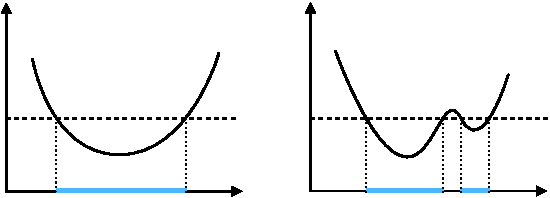
\includegraphics{part_2/chapter_3/figures/sublevels.pdf}};
		\node (fx1) at (-4,1.5) {$f(x)$};
		\node (fx2) at (1.2,1.5) {$f(x)$};
		\node (x1) at (-0.4,-1.7) {$x$};
		\node (x2) at (4.75,-1.7) {$x$};
		\node (alpha1) at (-4.8, -0.3) {$\alpha$};
		\node (alpha1) at (0.4, -0.3) {$\alpha$};
	\end{tikzpicture}
	\caption{The lower level sets $S_\alpha$ (in blue) of two functions, given a value of $\alpha$. Notice the nonconvexity of the level set of the nonconvex function (on the right)} \label{fig:sublevels}
\end{figure}

Notice that, for convex functions, no discontinuity can be observed, making $S_\alpha$ convex. Lemma \ref{lem:level_sets} states this property.

\begin{lemma}\label{lem:level_sets}
	Let $S \subseteq \reals^n$ be a nonempty convex set and $f:S \mapsto \reals$ a convex function. Then, any level set $S_\alpha$ with $\alpha \in \reals$ is convex. 
\end{lemma} 
%
\begin{proof}
	Let $x_1, x_2 \in S_\alpha$. Thus, $x_1, x_2 \in S$ with $f(x_1) \leq \alpha$ and $f(x_2) \leq \alpha$. Let $\lambda \in (0,1)$ and $x = \lambda x_1 + (1-\lambda)x_2$. Since $S$ is convex, we have that $x \in S$. Now, by the convexity of $f$, we have 
	$$ f(x) \leq \lambda f(x_1) + (1 - \lambda)f(x_2) \leq \lambda\alpha + (1 - \lambda)\alpha = \alpha
	$$
	and thus $x \in S_\alpha$.
\end{proof}

{\bf Remark:} notice that a convex lower level set does not necessarily mean that the function is convex. In fact, as we will see later, there are nonconvex functions that have convex level sets (the so-called quasiconvex functions).  

\subsection{Convex functions and their epigraphs}

\emph{Epigraphs}, on the other hand, can be used to show the convexity of functions. Let us first formally define epigraphs.
%
\begin{definition}[Ephigraph]
	Let $S \subseteq \reals^n$\hspace{-1pt} be a nonempty set and $f:S \mapsto \reals$.\hspace{-1pt} The epigraph of $f$ is $$ \epi(f) = \braces{(x, y) : x \in S, y \in \reals, y \geq f(x)} \subseteq \reals^{n+1}
$$
\end{definition}
%
Figure \ref{fig:epigraphs} illustrates the epigraphs of two functions. Notice that the second function (on the right) is not convex, and nor is its epigraph. In fact, we can use the convexity of epigraphs (and the technical results associated with the convexity of sets) to show the convexity of functions.
% 
\begin{figure}
	\begin{tikzpicture}
%		\draw[help lines] (-6,-2) grid (6,2);
		\node (pic) at (0,0) {	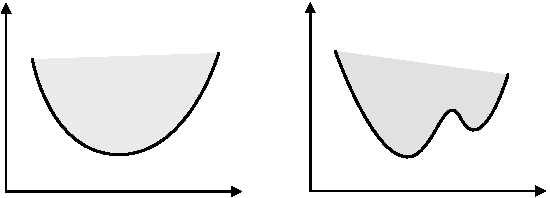
\includegraphics{part_2/chapter_3/figures/epigraphs.pdf}}; 		
		\node (fx1) at (-4,1.5) {$f(x)$};
		\node (fx2) at (1.2,1.5) {$f(x)$};
		\node (x1) at (-0.4,-1.7) {$x$};
		\node (x2) at (4.75,-1.7) {$x$};
		\node (epi1) at (-2.5, 0) {$\epi(f)$};				
		\node (epi2) at (2.5, 0.2) {$\epi(f)$};
	\end{tikzpicture}
	\caption{The epigraph $\epi()f$ of a convex function is a convex set (in grey on the left).}\label{fig:epigraphs}
\end{figure}
%
\begin{theorem}[Convex epigraphs]\label{thm:convex_epi}
	Let $S \subseteq \reals^n$ be a nonempty convex set and $f:S \mapsto \reals$. Then $f$ is convex if and only if $\epi(f)$ is a convex set.
\end{theorem}
%
\begin{proof}
	First, suppose $f$ is convex and let $(x_1, y_1), (x_2, y_2)$ $\in \epi(f)$ for $\lambda \in (0,1)$. Then
\begin{equation*}
	\lambda y_1 + (1-\lambda)y_2 \geq \lambda f(x_1) + (1-\lambda)f(x_2) \geq f(\lambda x_1 + (1- \lambda)x_2).
\end{equation*}
As $\lambda x_1 + (1-\lambda)x_2 \in S$, $(\lambda x_1 + (1-\lambda)x_2,\lambda y_1 + (1-\lambda)y_2) \in \epi(f)$.

Conversely, suppose $\epi(f)$ is convex. Therefore $x_1, x_2 \in S$: $(x_1,f(x_1))\in \epi(f)$, $(x_2,f(x_2)) \in \epi(f)$ and $(\lambda x_1 + (1-\lambda)x_2, \lambda f(x_1) + (1-\lambda)f(x_2)) \in \epi(f)$ for $\lambda \in (0,1)$, implying that $\lambda f(x_1) + (1-\lambda)f(x_2) \geq f(\lambda x_1 + (1-\lambda)x_2)$.
\end{proof}

The proof starts with the implication ``if $f$ is convex, then $\epi(f)$ is convex''. For that, it assumes that $f$ is convex and use the convexity of $f$ to show that any convex combination of $x_1$,$x_2$ in $S$ will also be in the $\epi(f)$, which is the definition of a convex set.

To prove the implication ``if $\epi(f)$ is convex, then $f$ is convex'', we define a convex combination of points in $\epi(f)$ and use the definition of $\epi(f)$ to show that $f$ is convex by setting $y = \lambda f(x_1) + (1 - \lambda)f(x_2)$ and $x = \lambda x_1 + (1-\lambda)x_2$.


\section{Differentiability of functions}


\subsection{Subgradients and supporting hyperplanes}


Subgradients can be understood as supporting hyperplanes at the boundary of function epigraphs. They can be seem as first-order local approximations of the function, which is often helpful information for optimisation methods when searching for directions of improvement.
%
\begin{definition}[Subgradients]
	Let $S \subseteq \reals^n$ be a nonempty convex set and $f:S \mapsto \reals$ a convex function. Then $\xi\in \reals^n$ is a \emph{subgradient} of $f$ at $\overline{x} \in S$ if
	\begin{align} 
	f(x) \geq f(\overline{x}) + \xi^\top(x - \overline{x}). \label{eq:subgradient_inequality}
	\end{align}
\end{definition}
%
Inequality \eqref{eq:subgradient_inequality} is called the \emph{subgradient inequality} and is going to be useful in several contexts later int his course. The set of subgradients $\xi$ of $f$ at $\overline{x}$ is the \emph{subdifferential} 
	$$
	\partial_f(\overline{x}) = \braces{\xi \in \reals^n : f(x) \geq f(\overline{x}) + \xi^\top(x - \overline{x})}.
	$$ 

Every convex function $f : S \mapsto \reals$ has at least one subgradient at any point $\overline{x}$ in the interior of the convex set $S$. Requiring that $\overline{x} \in \intr(S)$ allows us to disregard boundary points of $f$ where $\partial(\overline{x})$ might be empty. Theorem \ref{thm:exist_subgrad} presents this result.
%
\begin{theorem}\label{thm:exist_subgrad}
	Let $S \subseteq \reals^n$ be a nonempty convex set and $f:S \mapsto \reals$ a convex function. Then for all $\overline{x} \in \intr(S)$, there exists $\xi\in \reals^n$ such that
	$$ H = \braces{(x,y) : y = f(\overline{x}) + \xi^\top(x - \overline{x})}$$ supports $\epi(f)$ at $(\overline{x}, f(\overline{x}))$. In particular,
	$$f(x) \geq f(\overline{x}) + \xi^\top(x - \overline{x}), \forall x \in S.$$
\end{theorem}
%
The proof consists of directly applying Theorem \ref {thm:convex_epi} and then using the support of convex sets theorem (Theorem 14 in Lecture 2) to show that the subgradient inequality holds.

% Add the actual proof for this.

\subsection{Differentiability and gradients for convex functions} 


Let us first define differentiability of a function.
%
\begin{definition}
	Let $S \subseteq \reals^n$ be a nonempty set. The function $f:S \mapsto \reals$ is differentiable at $\overline{x} \in \intr(S)$ if there exists a vector $\nabla f(\overline{x})$, called a gradient vector, and a function $\alpha: \reals^n \mapsto \reals$ such that 
	$$
	f(x) = f(\overline{x}) + \nabla f(\overline{x})^\top(x - \overline{x}) + ||x-\overline{x}||\alpha(\overline{x};x-\overline{x})
	$$ 
	where $\lim_{x \mapsto \overline{x}}\alpha(\overline{x}; x - \overline{x})=0$. If this is the case for all $\overline{x} \in \intr(S)$, we say that the function is differentiable in $S$.
\end{definition}
%
Notice that this definition is based on the existence of first-order (Taylor series) expansion, with an error term $\alpha$. This definition is useful as it highlights the requirement that $\nabla f(\overline{x})$ exists and is unique at $\overline{x}$ since the gradient is given by $\nabla f(x) = \left[ \frac{\partial f(x)}{\partial x_i} \right]_i=1,\dots,n$. 

If $f$ is differentiable in $S$, then its subdifferential $\partial(x)$ is a singleton (a set with a single element) for all $x \in S$. This is shown in Lemma \ref{lem:singleton_subgradient}
%
\begin{lemma}\label{lem:singleton_subgradient}
	Let $S \subseteq \reals^n$ be a nonempty convex set and $f:S \mapsto \reals$ a convex function. Suppose that $f$ is differentiable at $\overline{x} \in \intr(S)$. Then $\partial_f(\overline{x}) = \braces{\nabla f(\overline{x})}$, i.e., the subdifferential $\partial_f(\overline{x})$ is a singleton with $\nabla f(\overline{x})$ as its unique element.
\end{lemma}
%
\begin{proof}
	From Theorem \ref{thm:exist_subgrad}, $\partial f(\overline{x}) \neq \emptyset$. Moreover, combining the existence of a subgradient $\xi$ and differentiability of $f$ at $\overline{x}$, we obtain:
	\begin{align}
	&f(\overline{x} + \lambda d) \geq f(\overline{x}) + \lambda \xi^\top d \label{1}\\
	&f(\overline{x} + \lambda d) = f(\overline{x}) + \lambda \nabla f(\overline{x})^\top d + \lambda ||d||\alpha(\overline{x}; \lambda d) \label{2}
	\end{align}
	Subtracting \eqref{2} from \eqref{1}, we get 
	$
	0 \geq \lambda(\xi - \nabla f(\overline{x}))^\top d -\lambda ||d||\alpha(\overline{x}; \lambda d).
	$
	Dividing by $\lambda > 0$ and letting $\lambda \mapsto 0^+$, we obtain $(\xi - \nabla f(\overline{x}))^\top d \leq 0$. Now, by setting $d = \xi - \nabla f(\overline{x})$, it becomes clear that $\xi = \nabla f(\overline{x})$.
\end{proof}

Notice that in the proof we use $\overline{x} + \lambda d$ to indicate that $x$ is in direction $d$, scaled by $\lambda > 0$. The fact that $\partial_f(x)$ is a singleton comes from the uniqueness of the solution for $(\xi - \nabla f(\overline{x}))^\top(\xi - \nabla f(\overline{x})) = 0$.

Figure \ref{fig:subgradients} illustrates subdifferential sets for three distinct points of a piecewise linear function. The picture schematically represents a multidimensional space $x$ as a one-dimensional projection (you can imagine this picture as being a section in one of the $x$ dimensions). For the points in which the function is not differentiable, the subdifferential set contains an infinite number of subgradients. At points in which the function is differentiable (any mid-segment point) the subgradient is unique (a gradient) and the subdifferential is a singleton.

	\begin{figure}
		\begin{tikzpicture}
%			\draw[help lines] (-3.5,-3) grid (4,3); 
			\node (pic) at (0,0) {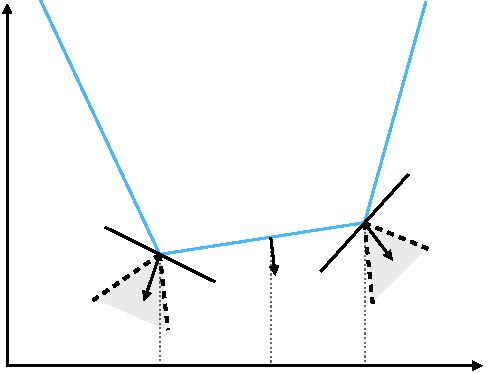
\includegraphics{part_2/chapter_3/figures/subgradients.pdf}};
			\node (fx) at (-4.5,3) {$f(x)$};
			\node (x) at (4.1,-3.2) {$x$};
			\node (xi1) at (-1.8,-2) {\footnotesize$\xi$};
			\node (xi2) at (2.55,-1.4) {\footnotesize$\xi$};
			\node (nablaf1) at (-2,-2.5) {$\partial f(x_1)$};
			\node (nablaf2) at (3,-1.9) {$\partial f(x_3)$};
			\node (nablaf3) at (0,-0.5) {\small$\partial f(x_2) = \nabla f(x_2)$};
			\node (x1) at (-1.4,-3.3) {$x_1$};
			\node (x2) at (0.5,-3.3) {$x_2$};
			\node (x3) at (2.1,-3.3) {$x_3$};	
		\end{tikzpicture}
		
		\caption{A representation of the subdifferential (in grey) for nondifferentiable ($x_1$ and $x_3$) and differentiable ($x_2$) points}\label{fig:subgradients}
	\end{figure}




If $f:S \mapsto \reals$ is a convex differentiable function, then Theorem \ref{thm:exist_subgrad} can be combined with Lemma \ref{lem:singleton_subgradient} to express the one of the most powerful results relating $f$ and its affine (first-order) approximation at $\overline{x}$.
%
\begin{theorem}[Convexity of a function II]\label{thm:convex_affine_bound}
	Let $S \subseteq \reals^n$ be a nonempty convex open set, and let $f:S \mapsto \reals$ be differentiable on $S$. The function $f$ is convex if and only if for any $\overline{x} \in S$, we have
	%
	\begin{align*}
		f(x) \geq f(\overline{x}) + \nabla f(\overline{x})^\top(x - \overline{x}), ~\forall x \in S.
	\end{align*}
\end{theorem}
%
The proof for this theorem follows from the proof for Theorem \ref{thm:exist_subgrad} to obtain the subgradient inequality and then use Lemma \ref{lem:singleton_subgradient} to replace the subgradient with the gradient. To see how the opposite direction (subgradient inequality holing implying the convexity of $f$), one should proceed as follows. 
\begin{enumerate}
	\item Take $x_1$ and $x_2$ from $S$. The convexity of $S$ implies that $\lambda x_1 + (1-\lambda)x_2$ is also in $S$.
	\item Assume that the subgradient exists, and therefore the two relations hold:
	%
	\begin{align}
		& f(x_1) \ge f(\lambda x_1 + (1-\lambda )x_2) + (1-\lambda )\xi^\top (x_1- x_2) \label{eq:conv1} \\
		& f(x_2) \ge f(\lambda x_1 + (1-\lambda )x_2) + \lambda \xi^\top (x_2- x_1) \label{eq:conv2}
	 \end{align}
	 \item Multiply \eqref{eq:conv1} by $\lambda$, \eqref{eq:conv2} by $(1-\lambda)$, and add them together. One will then obtain
	$$\lambda f(x_1) + (1-\lambda)f(x_2) \ge f(\lambda x_1 + (1-\lambda )x_2),$$ which is implies convexity.	 
\end{enumerate}



\subsection{Second-order differentiability}

 
We say that a function is \emph{twice-differentiable} if it has a second-order Taylor expansion. Having second-order expansions can be useful in that it allows for encoding curvature information in the approximation, which is characterised by the \emph{Hessian}, and to verify convexity (or strict convexity) by testing for semi-definiteness (positive definiteness).

Let $f_{ij}(\overline{x}) = \frac{\partial^2f(\overline{x})}{\partial x_i\partial x_j }$. Recall that the Hessian matrix  $H(\overline{x})$ at $\overline{x}$ is given by
%
\begin{align*}H(\overline{x}) = 
	\begin{bmatrix}
	f_{11}(\overline{x}) & \dots & f_{1n}(\overline{x})\\
	\vdots & \ddots & \vdots\\
	f_{n1}(\overline{x}) & \dots & f_{nn}(\overline{x})
	\end{bmatrix}
\end{align*}
%
Second-order differentiability can be defined as follows.
%
\begin{definition}[Second-order differentiability]
	Let $S \subseteq \reals^n$ be a nonempty set, and let $f:S \mapsto \reals$. Then $f$ is twice differentiable at $\overline{x} \in \intr(S)$ if there exists a vector $\nabla f(\overline{x})\in \reals^n$, an $n \times n$ symmetric matrix $H(\overline{x})$ (the Hessian), and a function $\alpha: \reals^n \mapsto \reals$ such that 
	\begin{align*}
	f(x) = f(\overline{x}) + \nabla f(\overline{x})^\top(x - \overline{x}) + 
	\frac{1}{2}(x - \overline{x})^\top H(\overline{x})(x - \overline{x}) + 
	||x-\overline{x}||^2\alpha(\overline{x};x-\overline{x})
	\end{align*}
	%
	where $\lim_{x \mapsto \overline{x}}\alpha(\overline{x}; x - \overline{x})=0$. If this is the case for all $\overline{x} \in S$, we say that the function is twice differentiable in $S$.
\end{definition}
%
We say that $H(\overline{x})$ is \emph{positive semi-definite} if $x^\top H(\overline{x})x \geq 0$ for $x \in \reals^n$. Having a positive semi-definite Hessian for all $x \in S$ implies that the function is convex in $S$. 
%
\begin{theorem}
	Let $S \subseteq \reals^n$ be a nonempty convex open set, and let $f:S \mapsto \reals$ be twice differentiable on $S$.\hspace{-4pt} Then\hspace{-1pt} $f$\hspace{-1pt} is convex if and only if the Hessian matrix is positive semidefinite (PSD) at each point in $S$.
\end{theorem}
%
\begin{proof}
Suppose $f$ is convex and let $\overline{x} \in S$. Since $S$ is open, $\overline{x} + \lambda x \in S$ for a small enough $|\lambda| \neq 0$. From Theorem \ref{thm:convex_affine_bound} and twice differentiability of $f$, we have 
%
\begin{align}
	&f(\overline{x} + \lambda x) \geq f(\overline{x}) + \lambda\nabla f(\overline{x})^\top x \label{3}\\ 
	&f(\overline{x} + \lambda x) =  f(\overline{x}) + \lambda \nabla f(\overline{x})^\top x + \frac{1}{2}\lambda^2 x^\top H(\overline{x})x + \lambda^2||x||^2\alpha(\overline{x};\lambda x) \label{4}
\end{align}
%
Subtracting \eqref{3} from \eqref{4}, we get 
$\frac{1}{2}\lambda^2x^\top H(\overline{x})x + \lambda^2||x||^2\alpha(\overline{x}; \lambda x) \geq 0$. Diving by $\lambda^2 > 0$ and letting $\lambda \rightarrow 0$, it follows that $x^\top H(\overline{x})x \geq 0$.

Conversely, assume that $H(\overline{x})$ is PSD for all $\overline{x} \in S$. Using the mean value theorem and second-order expansion, one can show that
%
\begin{align*}
	f(x) = f(\overline{x}) + \nabla f(\overline{x})^\top(x - \overline{x}) + \frac{1}{2}(x-\overline{x})^\top H(\hat{x})(x - \overline{x})
\end{align*}
%
where $\hat{x} = \lambda \overline{x} + (1-\lambda) x$ for $\lambda \in (0,1)$. Note that $\hat{x} \in S$ and $H(\hat{x})$ is positive semidefinite by assumption. Thus \hspace{-2pt}$(x-\overline{x})^\top H(\hat{x})(x - \overline{x}) \geq 0$, implying $f(x) = f(\overline{x}) + \nabla f(\overline{x})^\top(x - \overline{x}) \geq 0$.
\end{proof}
%
The proof uses a trick we have seen before. First, we assume convexity and use the definition of convexity provided by Theorem \ref{thm:convex_affine_bound} combined with an alternative definition for $(x - \overline{x})$ to show that $x^\top H(\overline{x})x \geq 0$. That is, instead of using the reference points $x$ and $\overline{x}$, we incorporate a step size $\lambda$ from $\overline{x}$ in the direction of $x$. 

To show the other direction of implication, that is, that $x^\top H(\overline{x})x \geq 0$ implies convexity, we use the \emph{mean value theorem}. The mean value theorem states that there must exist a point $\hat{x}$ between $x$ and $\overline{x}$ for which the second order approximation is exact. From these, we can derive the definition of convexity, as in Theorem \ref{thm:convex_affine_bound}.

Checking for positive semi-definiteness can be done efficiently using appropriate computational algebra method, though it can be computationally expensive. It involves calculating the eigenvalues of $H(\overline{x})$ and testing whether they are all nonnegative (positive), which implies the positive semi-definiteness (definiteness) of $H(\overline{x})$. Some nonlinear solvers are capable of returning warning messages (or errors even) pointing out lack of convexity by testing (under a certain threshold) for positive semi-definiteness.


\section{Quasiconvexity}

Quasiconvexity can be seem as the generalisation of convexity to functions that are not convex, but share similar properties that allow for defining global optimality conditions. One class of these functions are named \emph{quasiconvex}. Let us first technically define quasiconvex functions.
%
\begin{definition}[quasiconvex functions]
	Let $S \subseteq \reals^n$ be a nonempty convex set and $f:S \mapsto \reals$. Function $f$ is quasiconvex if, for each $x_1 ,x_2 \in S$ and $\lambda \in (0,1)$, we have
	\begin{align}
		f(\lambda x_1 + (1 - \lambda)x_2 ) \leq \max\braces{f(x_1), f(x_2)}. \label{eq:quasiconvexity}
	\end{align}
\end{definition}

We say that, if $f$ is quasiconvex, then $-f$ is quasiconcave. Also, functions that are both quasiconvex and quasiconcave are called \emph{quasilinear}. Quasiconvex functions are also called \emph{unimodal}.

Figure \ref{fig:quasiconvex} illustrates a quasiconvex function. Notice that, for any pair of points $x_1$ and $x_2$ in the domain of $f$, the graph of the function is always below the maximum between $f(x_1)$ and $f(x_2)$. This is precisely what renders convex the lower level sets of quasiconvex functions. Notice that, on the other hand, the epigraph $epi(f)$ is not a convex set. 

\begin{figure}[H]
		\begin{tikzpicture}
	%		\draw[help lines] (-6,-2) grid (6,2);
			\node (pic) at (0,0) {	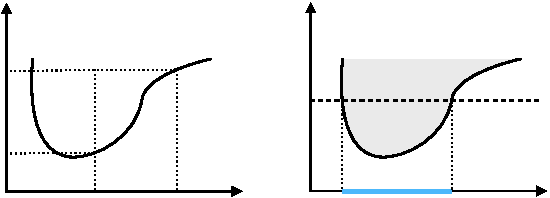
\includegraphics{part_2/chapter_3/figures/quasiconvex}}; 		
			\node (fx1) at (-4,1.5) {$f(x)$};
			\node (fx2) at (1.2,1.5) {$f(x)$};
			\node (x1) at (-0.4,-1.7) {$x$};
			\node (x2) at (4.75,-1.7) {$x$};
			\node (x11) at (-3, -1.8) {$x_1$};				
			\node (x21) at (-1.6, -1.8) {$x_2$};
	 		\node (fx11) at (-5.1, -0.9) {$f(x_1)$};
	  		\node (fx21) at (-5.1, 0.5) {$f(x_2)$};
	  		\node (fx21) at (0.3, 0) {$\alpha$};
	  		\node (fx21) at (2,-1.8) {$S_\alpha$};			
		\end{tikzpicture}
		\caption{A quasiconvex function with its epigraph (in grey) and lower level set (in blue).} \label{fig:quasiconvex}
	\end{figure}



Examples of quasiconvex functions include:
%
\begin{enumerate}
	\item $f(x) = \sqrt{|x|}$ in $\reals$
	\item $f(x) = \log x$ is quasilinear for $x > 0 $ 
	\item $f(x) = \inf\braces{z \in \integers : z \geq x}$ is quasilinear
	\item $f(x_1,x_2) = x_1x_2$ is quasiconcave on $S = \braces{(x_1, x_2) \in \reals^2 : x_1,x_2 > 0}$
\end{enumerate}
%
An important property of quasiconvex functions is that their level sets are convex. 
%
\begin{theorem}
	Let $S \subseteq \reals^n$ be a nonempty convex set and $f:S \mapsto \reals$. Function $f$ is quasiconvex if and only if $S_\alpha = \braces{x \in S: f(x) \leq \alpha}$ is convex for all $\alpha \in \reals$.
\end{theorem}
%
\begin{proof}
	Suppose $f$ is quasiconvex and let $x_1, x_2 \in S_\alpha$. Thus, $x_1, x_2 \in S$ and $\max\braces{f(x_1), f(x_2)} \leq \alpha$. Let $x = \lambda x_1 + (1-\lambda)x_2$ for $\lambda \in (0,1)$. As $S$ is convex, $x \in S$. By quasiconvexity of $f$, $f(x) \leq \max\braces{f(x_1), f(x_2)} \leq \alpha$. Hence, $x \in S_\alpha$ and $S_\alpha$ is convex.  

	Conversely, assume that $S_\alpha$ is convex for $\alpha \in \reals$. Let $x_1, x_2 \in S$, and let $x = \lambda x_1 + (1-\lambda)x_2$ for $\lambda \in (0,1)$. Note that, for $\alpha = \max\braces{f(x_1), f(x_2)}$, we have $x_1, x_2 \in S_\alpha$. The convexity of $S_\alpha$ implies that $x \in S_\alpha$, and thus $f(x) \leq \alpha = \max\braces{f(x_1), f(x_2)}$, which implies that $f$ is quasiconvex.
\end{proof}
 
The proof relies on the convexity of the domain $S$ to show that a convex combination from point in the level set $S_\alpha$ also belongs to $S_\alpha$. To show the other way around, we simply need to define $\alpha = \max\braces{f(x_1), f(x_2)}$ to see that a convex level set $S_\alpha$ implies that $f$ is quasiconvex. 

Quasiconvex functions have an interesting first-order condition that arises from the convexity of its level sets.

\begin{theorem}\label{thm:first-order_quasiconvex}
Let $S \subseteq \reals^n$ be a nonempty open convex set, and let $f:S \mapsto \reals$\lb be differentiable on $S$. Then $f$ is quasiconvex if and only if, for $x_1, x_2 \in S$ and $f(x_1) \leq f(x_2)$, $\nabla f(x_2)^\top(x_1 - x_2) \leq 0$.
\end{theorem}
%
\begin{figure}[h]
	\begin{subfigure}[b]{0.45\textwidth}
		\includegraphics[width=\textwidth]{part_2/chapter_3/figures/quasiconvex_surface.pdf}\caption{surface plot}\label{fig:quasiconvex_surface}
	\end{subfigure}
	\begin{subfigure}[b]{0.45\textwidth}
		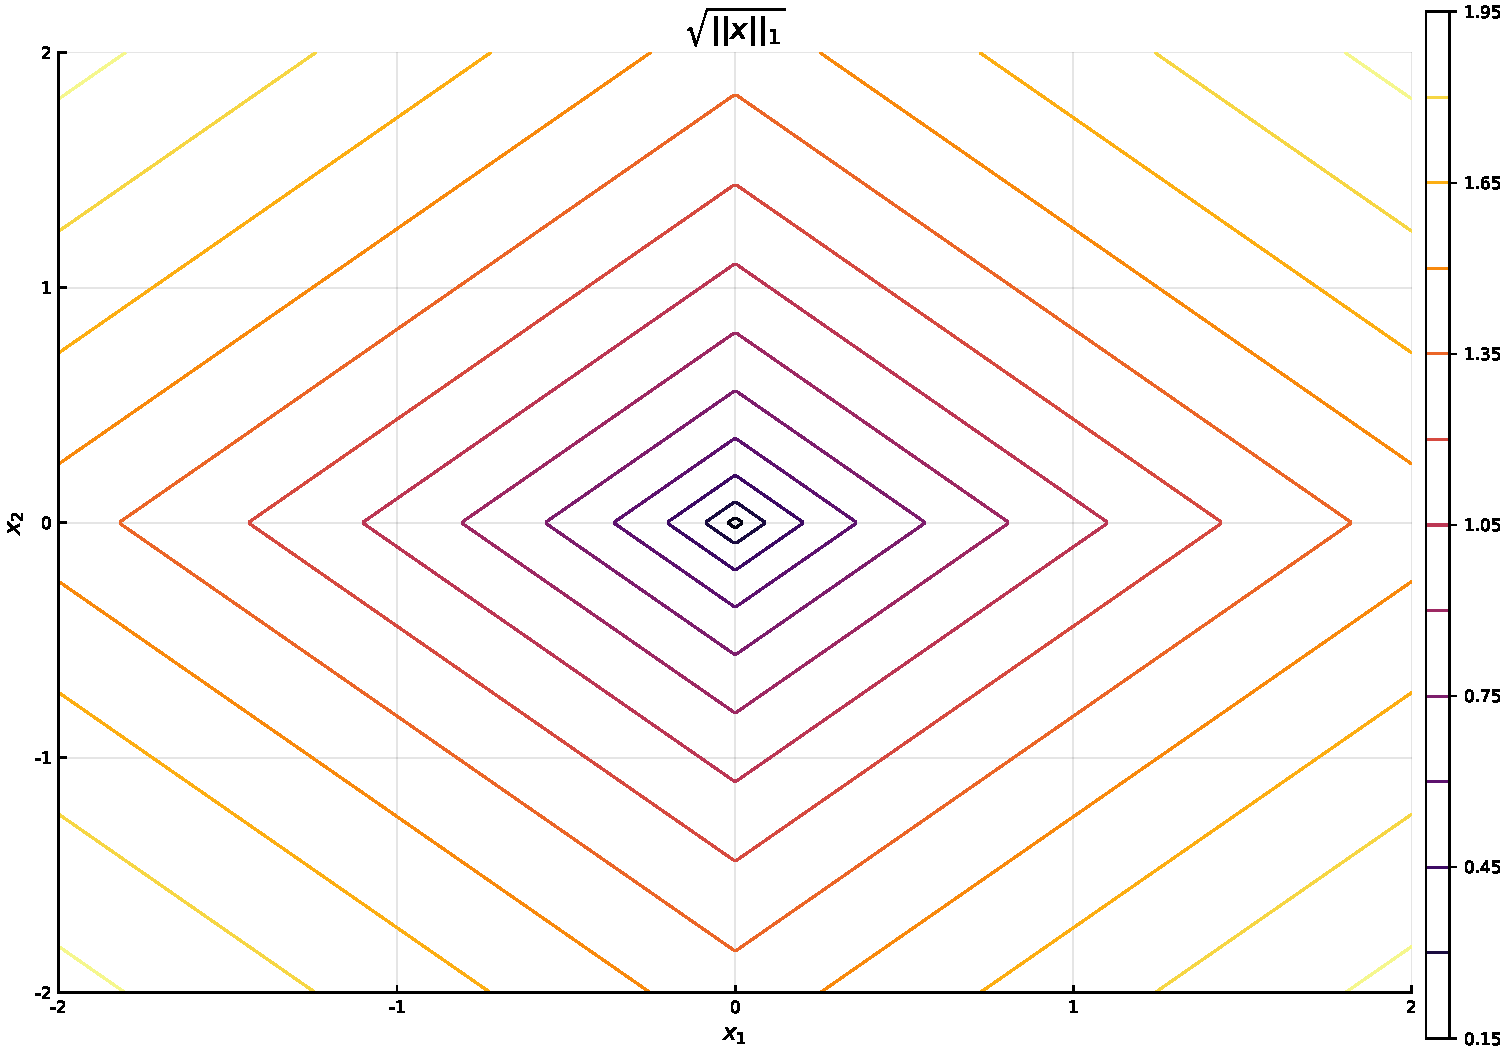
\includegraphics[width=\textwidth]{part_2/chapter_3/figures/quasiconvex_contours.pdf}
	\caption{level curves}\label{fig:quasiconvex_contours}
	\end{subfigure}
	\caption{Surface plot and level curves for $f(x) = \sqrt{||x||_1}$} 
\end{figure}

The condition in Theorem \ref{thm:first-order_quasiconvex} is in fact sufficient for global optimality if one can show that $f$ is in fact \emph{strictly quasiconvex}, that is when \eqref{eq:quasiconvexity} holds strictly. Figure \ref{fig:quasiconvex_surface} and \ref{fig:quasiconvex_contours} show an example of a strict quasiconvex function and its level curves, illustrating that, despite the lack of convexity, the level sets are convex.

Strictly quasiconvex functions is a subset of a more general class of functions named \emph{pseudoconvex}, for which the conditions in Theorem \ref{thm:first-order_quasiconvex} are sufficient for global optimality. 